\documentclass{standalone}

\usepackage[utf8]{inputenc}
\usepackage{tikz}

\begin{document}

% first method
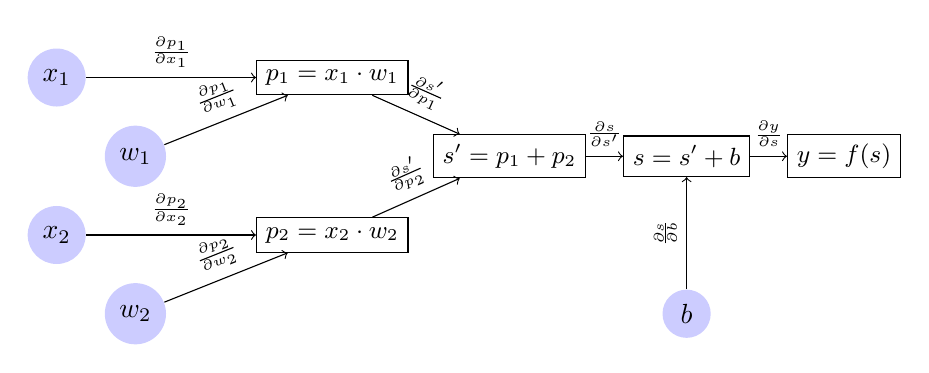
\begin{tikzpicture}[auto, node distance=3cm,
                    node_style/.style={circle,fill=blue!20},
                    edge_style/.style={->, draw=black, sloped, above},
                    sq/.style={draw, font=\small}
   ]
   \node[node_style] (x2) at (0,0) {$x_2$};
   \node[node_style] (x1) at (0,2) {$x_1$};
   \node[node_style] (w2) at (1,-1) {$w_2$};
   \node[node_style] (w1) at (1,1) {$w_1$};
   \node[node_style] (b) at (8, -1) {$b$};
   % Operations
   \node[sq] (p2) at (3.5,0) {$p_2 = x_2 \cdot w_2$};
   \node[sq] (p1) at (3.5,2) {$p_1 = x_1 \cdot w_1$};
   \node[sq] (sp) at (5.75,1) {$s' = p_1 + p_2$};
   \node[sq] (s) at (8,1) {$s = s' + b$};
   \node[sq] (y) at (10,1) {$y = f(s)$};

    \draw[edge_style]  (x1) edge node{\tiny $\frac{\partial p_1}{\partial x_1}$} (p1);
    \draw[edge_style]  (w1) edge node{\tiny $\frac{\partial p_1}{\partial w_1}$} (p1);
    \draw[edge_style]  (x2) edge node{\tiny $\frac{\partial p_2}{\partial x_2}$} (p2);
    \draw[edge_style]  (w2) edge node{\tiny $\frac{\partial p_2}{\partial w_2}$} (p2);
    \draw[edge_style]  (p1) edge node{\tiny $\frac{\partial s'}{\partial p_1}$} (sp);
    \draw[edge_style]  (p2) edge node{\tiny $\frac{\partial s'}{\partial p_2}$} (sp);
    \draw[edge_style]  (b) edge node{\tiny $\frac{\partial s}{\partial b}$} (s);
    \draw[edge_style]  (sp) edge node{\tiny $\frac{\partial s}{\partial s'}$} (s);
    \draw[edge_style]  (s) edge node{\tiny $\frac{\partial y}{\partial s}$} (y);
    \end{tikzpicture}
\end{document}
